\subsubsection{Tag Rate Function method}\label{sec:trf}

When requiring $\geq 1$ $b$-tagged jet the
available Monte Carlo statistics is significantly reduced for 
some particular background processes, leading to large
fluctuations in the resulting distributions.
% This can negatively
%affect the sensitivity of the analysis, as the corresponding
%statistical uncertainties on the background templates need to be taken
%into account in the determination of exclusion limits, and lead to
%unreliable systematic uncertainties in the predicted distribution
%shapes. In addition, the observed limits may be biased, depending on
%how the MC distributions fluctuate with respect to the data in the
%signal region.


To overcome this problem the Tag Rate Function (TRF) method is introduced.
Here, no event is rejected based on its $b$-tagging count, but instead all the events are 
kept and weighted according to the
probability of the given event to contain the desired number of \bjet s.
The event weight is computed based on the kinematics and flavour of the jets found in each event
and using the tagging efficiency, which is a function of $\eta$, $\pt$ and true jet flavour.

Given a jet with $\eta$, $\pt$ and flavour $f$, its tagging probability can be noted as:
\begin{equation*}
        \varepsilon \left(f,|\eta|,\pt\right)
\end{equation*}

For a given event with $N$ jets, its probability of containing exactly one $b$-tag jet can be computed as:
\begin{equation*}
        P_{=1} = \sum\limits_{i=1}^N \left( \varepsilon_{i} \prod\limits_{i \neq j} \left( 1 - \varepsilon_{j} \right) \right)
\end{equation*}

In the same way, it can be used to compute the probability for inclusive $b$-tag selections:
\begin{align*}
        P_{=0} &= \prod\limits_{i=1}^N \left( 1 - \varepsilon_{j} \right) \\
        P_{\geq 1} &= 1 - P_{=0}
\end{align*}

Since this method relies on the correctness of the tagging efficiency,  closure tests have been performed to check
calibration of the tagging efficiency in Monte Carlo samples. These studies show that the efficiency parametrization
officially provided~\cite{topcommon2013}  is not as accurate as expected, and therefore new efficiency maps where
obtained. With correct calibrations the average of the histogram of $1/\varepsilon$ vs $\eta$, $\pt$ and true jet flavour 
should be flat and with mean equal to one. Figure~\ref{fig:closure} shows these variables using the official and the new maps.
%As it can be observed, there are departures from closure of to up to 40\% in some regions of the light flavor map, and on average 13\%.
%New efficiency maps have been derived using a combination of $t\bar{t}$ {\sc MC@NLO}, $t\bar{t}$ {\sc Alpgen}, and {\sc Protos} $\TT$ MC samples.
%Figure~\ref{fig:closure} shows reasonably good closure for the newly derived efficiency map.
%The new efficiency map will therefore be used for the probability computations in the TRF method.
It is clear that some regions of the light flavor map show high departure from closure, hence the
new efficiency map will be used for the probability computations in the TRF method.

\begin{figure}
  \begin{center}
  \begin{tabular}{c c}
    \includegraphics[width=0.45\textwidth]{objectsreconstruction/figures/TRFmethod/5closureRebin.eps} &
    \includegraphics[width=0.45\textwidth]{objectsreconstruction/figures/TRFmethod/5myclosureRebin.eps} \\
    \includegraphics[width=0.45\textwidth]{objectsreconstruction/figures/TRFmethod/4closureRebin.eps} &
    \includegraphics[width=0.45\textwidth]{objectsreconstruction/figures/TRFmethod/4myclosureRebin.eps} \\
    \includegraphics[width=0.45\textwidth]{objectsreconstruction/figures/TRFmethod/0closureRebin.eps} &
    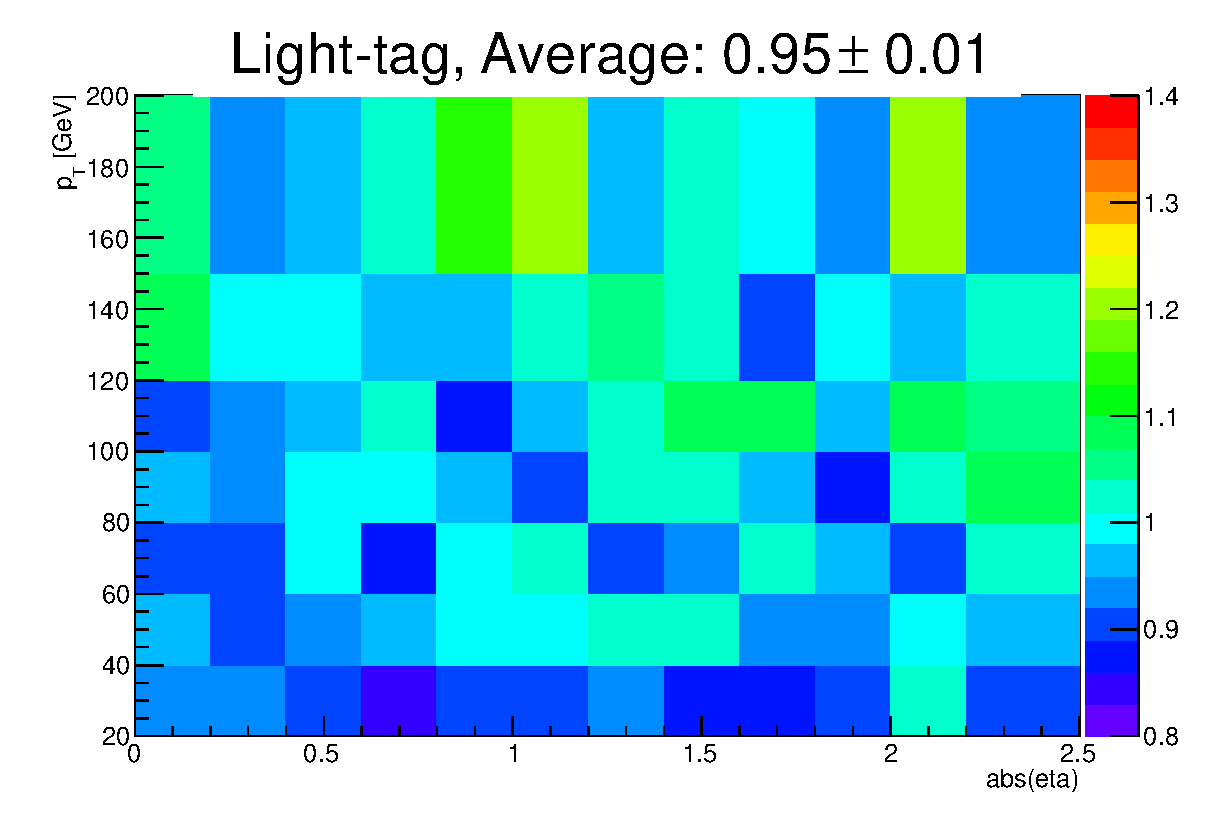
\includegraphics[width=0.45\textwidth]{objectsreconstruction/figures/TRFmethod/0myclosureRebin.eps} \\
  \end{tabular}
  \end{center}
  \caption{Results of the closure test using efficiency from the official calibration file 
  (left column) and the private efficiency map (right column). The test is split in the
 different jet flavours: $b$ jets (top), $c$ jets (middle) and light jets (bottom). }
  \label{fig:closure}
\end{figure}


